\documentclass[14pt]{extbook}
\usepackage{multicol, enumerate, enumitem, hyperref, color, soul, setspace, parskip, fancyhdr} %General Packages
\usepackage{amssymb, amsthm, amsmath, bbm, latexsym, units, mathtools} %Math Packages
\everymath{\displaystyle} %All math in Display Style
% Packages with additional options
\usepackage[headsep=0.5cm,headheight=12pt, left=1 in,right= 1 in,top= 1 in,bottom= 1 in]{geometry}
\usepackage[usenames,dvipsnames]{xcolor}
\usepackage{dashrule}  % Package to use the command below to create lines between items
\newcommand{\litem}[1]{\item#1\hspace*{-1cm}\rule{\textwidth}{0.4pt}}
\pagestyle{fancy}
\lhead{Progress Quiz 9}
\chead{}
\rhead{Version B}
\lfoot{8590-6105}
\cfoot{}
\rfoot{Fall 2020}
\begin{document}

\begin{enumerate}
\litem{
Describe the end behavior of the polynomial below.\[ f(x) = 5(x + 8)^{3}(x - 8)^{8}(x + 6)^{5}(x - 6)^{5} \]\begin{enumerate}[label=\Alph*.]
\begin{multicols}{2}\item 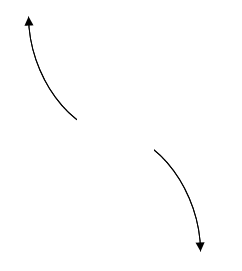
\includegraphics[width = 0.3\textwidth]{../Figures/polyEndBehaviorAB.png}\item 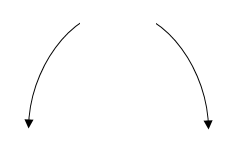
\includegraphics[width = 0.3\textwidth]{../Figures/polyEndBehaviorBB.png}\item 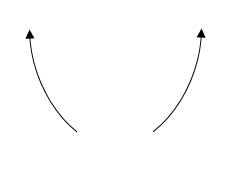
\includegraphics[width = 0.3\textwidth]{../Figures/polyEndBehaviorCB.png}\item 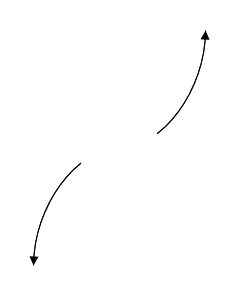
\includegraphics[width = 0.3\textwidth]{../Figures/polyEndBehaviorDB.png}\end{multicols}\item None of the above.
\end{enumerate} }
\litem{
Which of the following equations \textit{could} be of the graph presented below?
\begin{center}
    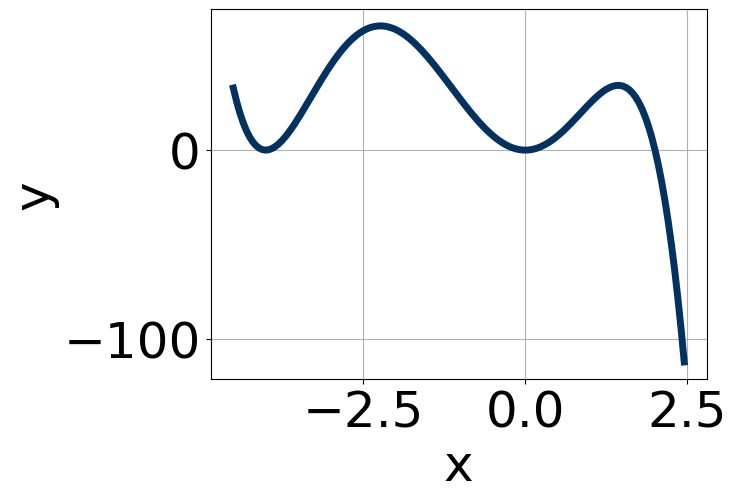
\includegraphics[width=0.5\textwidth]{../Figures/polyGraphToFunctionCopyB.png}
\end{center}
\begin{enumerate}[label=\Alph*.]
\item \( -20x^{8} (x - 1)^{4} (x + 4)^{5} \)
\item \( 14x^{5} (x - 1)^{4} (x + 4)^{4} \)
\item \( -7x^{6} (x - 1)^{5} (x + 4)^{9} \)
\item \( -3x^{5} (x - 1)^{6} (x + 4)^{11} \)
\item \( 20x^{7} (x - 1)^{10} (x + 4)^{11} \)

\end{enumerate} }
\litem{
Construct the lowest-degree polynomial given the zeros below. Then, choose the intervals that contain the coefficients of the polynomial in the form $ax^3+bx^2+cx+d$.\[ \frac{7}{2}, \frac{-4}{5}, \text{ and } -1 \]\begin{enumerate}[label=\Alph*.]
\item \( a \in [8, 21], b \in [14, 22], c \in [-56, -48], \text{ and } d \in [21, 32] \)
\item \( a \in [8, 21], b \in [32, 42], c \in [-1, 9], \text{ and } d \in [-30, -24] \)
\item \( a \in [8, 21], b \in [45, 61], c \in [65, 76], \text{ and } d \in [21, 32] \)
\item \( a \in [8, 21], b \in [-17, -10], c \in [-56, -48], \text{ and } d \in [21, 32] \)
\item \( a \in [8, 21], b \in [-17, -10], c \in [-56, -48], \text{ and } d \in [-30, -24] \)

\end{enumerate} }
\litem{
Construct the lowest-degree polynomial given the zeros below. Then, choose the intervals that contain the coefficients of the polynomial in the form $ax^3+bx^2+cx+d$.\[ \frac{4}{3}, \frac{-4}{5}, \text{ and } \frac{-5}{3} \]\begin{enumerate}[label=\Alph*.]
\item \( a \in [38, 47], b \in [-53, -46], c \in [-95, -81], \text{ and } d \in [75, 85] \)
\item \( a \in [38, 47], b \in [46, 59], c \in [-95, -81], \text{ and } d \in [-82, -72] \)
\item \( a \in [38, 47], b \in [46, 59], c \in [-95, -81], \text{ and } d \in [75, 85] \)
\item \( a \in [38, 47], b \in [96, 104], c \in [-8, 0], \text{ and } d \in [-82, -72] \)
\item \( a \in [38, 47], b \in [170, 174], c \in [208, 212], \text{ and } d \in [75, 85] \)

\end{enumerate} }
\litem{
Construct the lowest-degree polynomial given the zeros below. Then, choose the intervals that contain the coefficients of the polynomial in the form $x^3+bx^2+cx+d$.\[ 3 + 2 i \text{ and } 4 \]\begin{enumerate}[label=\Alph*.]
\item \( b \in [-3, 3], c \in [-7.24, -6.71], \text{ and } d \in [12, 18] \)
\item \( b \in [-17, -6], c \in [35.65, 38.84], \text{ and } d \in [-55, -51] \)
\item \( b \in [-3, 3], c \in [-6.62, -5.73], \text{ and } d \in [0, 11] \)
\item \( b \in [9, 11], c \in [35.65, 38.84], \text{ and } d \in [47, 55] \)
\item \( \text{None of the above.} \)

\end{enumerate} }
\litem{
Construct the lowest-degree polynomial given the zeros below. Then, choose the intervals that contain the coefficients of the polynomial in the form $x^3+bx^2+cx+d$.\[ -3 - 2 i \text{ and } -1 \]\begin{enumerate}[label=\Alph*.]
\item \( b \in [-1.4, 1.6], c \in [2.69, 3.9], \text{ and } d \in [0.87, 2.86] \)
\item \( b \in [-1.4, 1.6], c \in [3.53, 4.78], \text{ and } d \in [2.66, 3.65] \)
\item \( b \in [-7.8, -5.8], c \in [18.72, 19.42], \text{ and } d \in [-13.71, -12.62] \)
\item \( b \in [3.5, 10.6], c \in [18.72, 19.42], \text{ and } d \in [10, 13.23] \)
\item \( \text{None of the above.} \)

\end{enumerate} }
\litem{
Describe the zero behavior of the zero $x = -5$ of the polynomial below.\[ f(x) = 4(x + 5)^{6}(x - 5)^{11}(x - 6)^{6}(x + 6)^{9} \]\begin{enumerate}[label=\Alph*.]
\begin{multicols}{2}\item 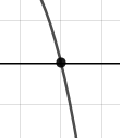
\includegraphics[width = 0.3\textwidth]{../Figures/polyZeroBehaviorCopyAB.png}\item 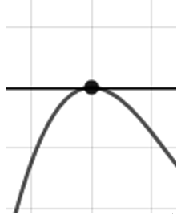
\includegraphics[width = 0.3\textwidth]{../Figures/polyZeroBehaviorCopyBB.png}\item 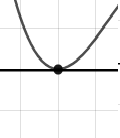
\includegraphics[width = 0.3\textwidth]{../Figures/polyZeroBehaviorCopyCB.png}\item 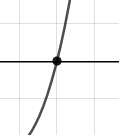
\includegraphics[width = 0.3\textwidth]{../Figures/polyZeroBehaviorCopyDB.png}\end{multicols}\item None of the above.
\end{enumerate} }
\litem{
Describe the end behavior of the polynomial below.\[ f(x) = -3(x - 9)^{5}(x + 9)^{6}(x - 3)^{4}(x + 3)^{6} \]\begin{enumerate}[label=\Alph*.]
\begin{multicols}{2}\item 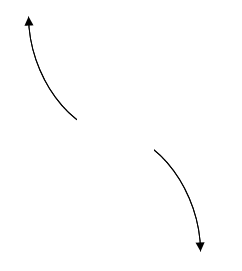
\includegraphics[width = 0.3\textwidth]{../Figures/polyEndBehaviorCopyAB.png}\item 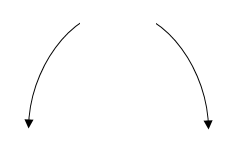
\includegraphics[width = 0.3\textwidth]{../Figures/polyEndBehaviorCopyBB.png}\item 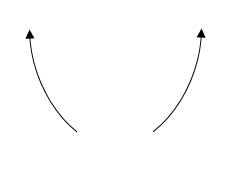
\includegraphics[width = 0.3\textwidth]{../Figures/polyEndBehaviorCopyCB.png}\item 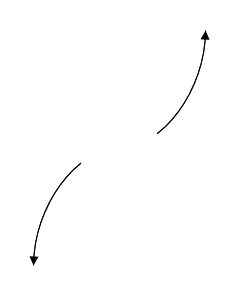
\includegraphics[width = 0.3\textwidth]{../Figures/polyEndBehaviorCopyDB.png}\end{multicols}\item None of the above.
\end{enumerate} }
\litem{
Which of the following equations \textit{could} be of the graph presented below?
\begin{center}
    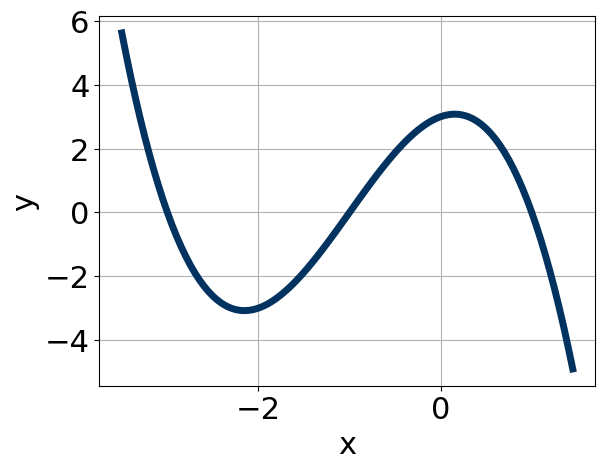
\includegraphics[width=0.5\textwidth]{../Figures/polyGraphToFunctionB.png}
\end{center}
\begin{enumerate}[label=\Alph*.]
\item \( -3(x + 1)^{10} (x + 2)^{8} (x - 2)^{11} \)
\item \( -19(x + 1)^{4} (x + 2)^{9} (x - 2)^{9} \)
\item \( 15(x + 1)^{4} (x + 2)^{10} (x - 2)^{9} \)
\item \( -5(x + 1)^{4} (x + 2)^{6} (x - 2)^{4} \)
\item \( 15(x + 1)^{4} (x + 2)^{8} (x - 2)^{4} \)

\end{enumerate} }
\litem{
Describe the zero behavior of the zero $x = 2$ of the polynomial below.\[ f(x) = 8(x - 7)^{6}(x + 7)^{3}(x - 2)^{6}(x + 2)^{3} \]\begin{enumerate}[label=\Alph*.]
\begin{multicols}{2}\item 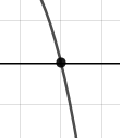
\includegraphics[width = 0.3\textwidth]{../Figures/polyZeroBehaviorAB.png}\item 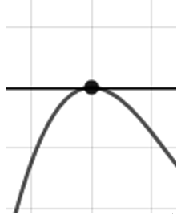
\includegraphics[width = 0.3\textwidth]{../Figures/polyZeroBehaviorBB.png}\item 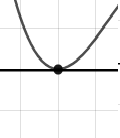
\includegraphics[width = 0.3\textwidth]{../Figures/polyZeroBehaviorCB.png}\item 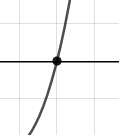
\includegraphics[width = 0.3\textwidth]{../Figures/polyZeroBehaviorDB.png}\end{multicols}\item None of the above.
\end{enumerate} }
\end{enumerate}

\end{document}